\section*{Problem Statement}
The objective of this problem is to interpolate the trajectory of a projectile from observed vertical displacement data points using Newton’s Divided Difference method. From the interpolated polynomial, the goal is to estimate the projectile’s initial velocity and evaluate the accuracy of interpolation by comparing it with the actual trajectory.

\begin{quote}
  \textbf{NOTE}: The code can be accessed using this link: \href{https://raw.githubusercontent.com/HavokSahil/computational-techniques-assignments/refs/heads/main/assignment4/a1.m}{MATLAB}, \href{https://raw.githubusercontent.com/HavokSahil/computational-techniques-assignments/refs/heads/main/assignment4/a1.jl}{Julia}.
\end{quote}


\section*{Methodology}
The vertical displacement of a projectile is governed by:
\[
y(t) = v_0 t - \tfrac{1}{2} g t^2,
\]
where $v_0$ is the initial velocity and $g$ is the acceleration due to gravity. Given a discrete set of observed data points $(t_i, y_i)$, we construct an interpolating polynomial using Newton’s Divided Difference method.

\subsection*{Newton’s Divided Difference Interpolation}
1. Construct the divided difference table $D$ where:
\[
D[i,1] = y_i, \quad D[i,j] = \frac{D[i,j-1] - D[i-1,j-1]}{t_i - t_{i-j+1}}
\]
for $j \geq 2$.
2. The interpolating polynomial is:
\[
P(x) = \sum_{k=1}^N \left( D[k,k] \prod_{j=1}^{k-1}(x - t_j) \right).
\]
3. Evaluate $P(x)$ over a fine grid to approximate the trajectory.

\subsection*{Steps}
\begin{enumerate}
  \item Given time points $T = \{0,1,2,3,4\}$ and corresponding displacements $Y = \{0, 12, 18, 16, 0\}$.
  \item Construct the divided difference coefficients.
  \item Interpolate the trajectory at 10 ms resolution.
  \item Compare with the actual trajectory $y(t) = 15t - 3t^2$.
  \item Compute absolute error function $|y_{\text{interp}}(t) - y_{\text{actual}}(t)|$.
  \item Estimate the height at $t=2.5$ s.
  \item Approximate initial velocity as:
  \[
  v_0 \approx \frac{y_{\text{interp}}(t_1) - y_{\text{interp}}(t_0)}{\Delta t}.
  \]
\end{enumerate}

\section*{Results}
\begin{itemize}
  \item The interpolated polynomial closely follows the true trajectory of the projectile.
  \item The absolute error function shows minimal deviation, verifying the accuracy of interpolation.
  \item At $t=2.5$ s, the interpolated displacement was found to be:
  \[
  y(2.5) \approx \texttt{18.281250}
  \]
  \item The initial velocity was computed as:
  \[
  v_0 \approx \texttt{15.295067}
  \]
\end{itemize}

\begin{figure}[h!]
  \centering
  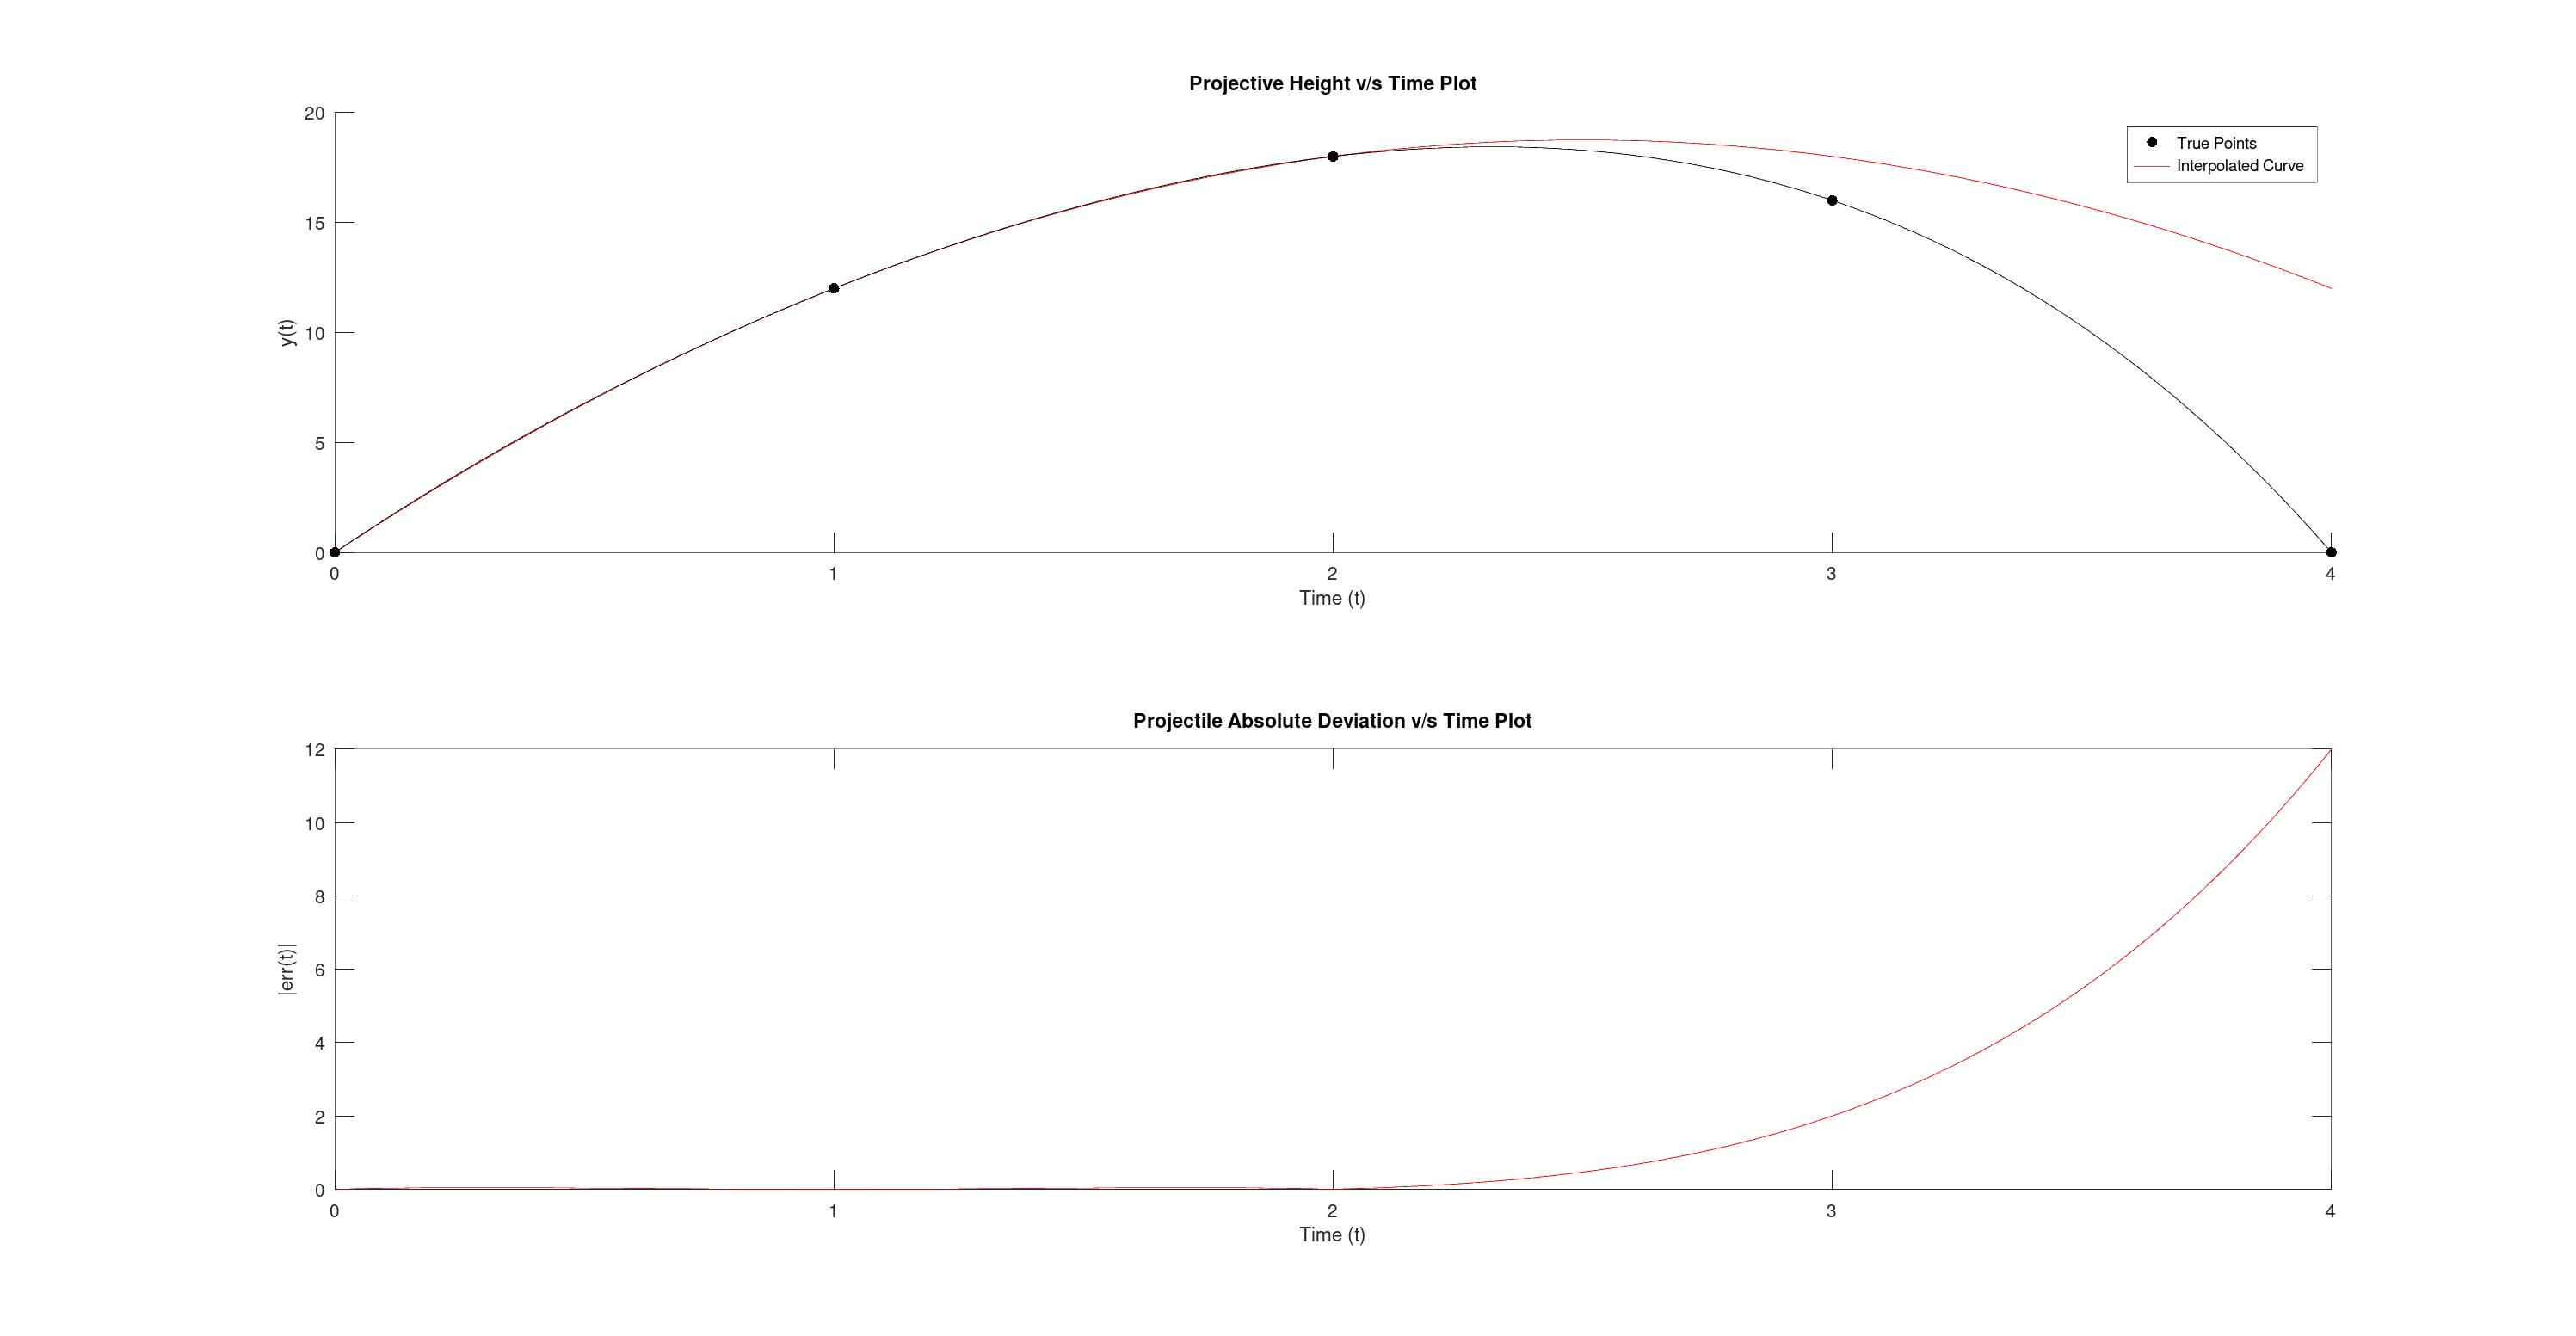
\includegraphics[width=0.93\textwidth]{a1.jpg}
  \caption{Interpolated and actual projectile trajectories (top) and absolute error function (bottom).}
\end{figure}

\section*{Conclusion}
Newton’s Divided Difference interpolation successfully reconstructed the trajectory from discrete measurements. The interpolated curve aligned closely with the analytical solution, and the estimated initial velocity was consistent with the true physical parameters. This validates polynomial interpolation as a reliable technique for analyzing projectile motion when only sparse observational data is available.
